\documentclass[cs4size,a4paper,nofonts]{ctexart}
\usepackage[utf8]{inputenc}
\def\tjf{田劲锋}
\def\titlec{智能手机操作系统}
\usepackage[top=25.4mm,bottom=25.4mm,left=31.8mm,right=31.8mm]{geometry} % 页面设置
\usepackage[unicode,breaklinks=true,
colorlinks=true,linkcolor=black,anchorcolor=black,citecolor=black,urlcolor=black,
pdftitle={\titlec},pdfauthor={\tjf}]{hyperref}
\usepackage{xeCJK}
\usepackage{xpinyin}

\usepackage{multicol} % 分栏
\usepackage{multirow} % 跨行
\usepackage{longtable} % 长表格
\usepackage{graphicx} % 图形
\usepackage{color} % 颜色
\usepackage{xcolor} % 颜色
\usepackage{url} % 排版链接
\usepackage{nameref}
\usepackage{caption}
\captionsetup{font={small}} % 标题字体大小
\usepackage[inline]{enumitem} % 调整列表样式

\setmainfont{Times New Roman}
\setCJKmainfont[BoldFont={SimHei}]{SimSun}  % 主要字体:宋体、黑体
\setCJKsansfont[BoldFont={STZhongsong}]{STFangsong} % 次要字体:仿宋、中宋
\setCJKmonofont{KFKai} % 等宽字体:楷体
\setCJKfamilyfont{msyh}[BoldFont={* Bold}]{微软雅黑} \newcommand{\msyh}{\CJKfamily{msyh}} % 微软雅黑
\setCJKfamilyfont{mincho}{MS PMincho} \newcommand{\mincho}{\CJKfamily{mincho}} % 文泉驿微米黑
\setCJKfamilyfont{fangso}{华文仿宋} \newcommand{\fangso}{\CJKfamily{fangso}} % STLiti
\setCJKfamilyfont{xingkai}{华文行楷} \newcommand{\xingkai}{\CJKfamily{xingkai}}

\CJKsetecglue{\hspace{0.1em}}
\renewcommand\CJKglue{\hskip -0.3pt plus 0.08\baselineskip}
\frenchspacing
\widowpenalty=10000
\linespread{1.5} % 1.5 倍行距
\setlength{\parskip}{2pt plus 2pt}
\renewcommand{\baselinestretch}{1.5}

\setlength{\abovecaptionskip}{1pt}
\setlength{\belowcaptionskip}{0pt}
\setlength{\intextsep}{8pt}
\setlist{topsep=0pt,partopsep=0pt,itemsep=0pt,parsep=0pt}

\makeindex
\pagestyle{plain}

\begin{document}

%%%% 开始 %%%%

\begin{titlepage}


\includegraphics[height=21.4mm]{images/hautlogo.png}
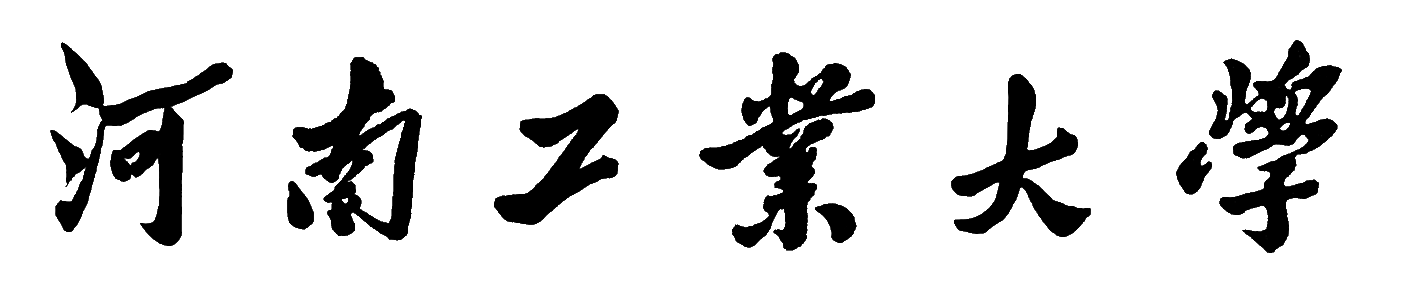
\includegraphics[height=20.4mm]{images/haut.png}

\begin{center}

\vspace*{1cm}

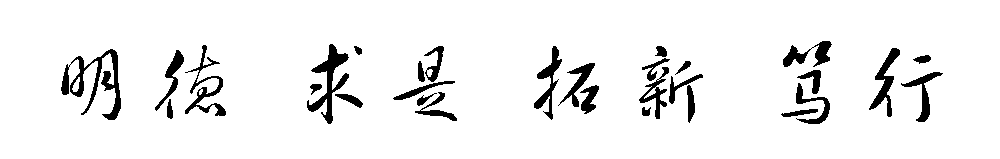
\includegraphics[height=25.1mm]{images/xiaoxun.png}

\vspace*{1cm}

{\xingkai\bfseries\zihao{1}{职业发展教育与就业指导}}

\vfill
{\large
\newcommand{\ctline}[2]{\makebox[4em][s]{\bf #1}:\underline{\makebox[15em][c]{#2}}\par}
\newcommand{\ctlin}[2]{\makebox[4em][s]{\bf #1}\quad\underline{\makebox[15em][c]{#2}}\par}
\ctline{题目}{\titlec}
\ctline{学院}{信息科学与工程学院}
\ctline{专业班级}{软件 1305 班}
\ctline{小组成员}{王飞飞~201316920312}
\ctlin{}{陆书航~201316920307}
\ctlin{}{马骁尧~201316920308}
\ctlin{}{王增辉~201316920309}
\ctlin{}{\makebox[3em][s]{陈辉}~201316920310}
\ctlin{}{\tjf~201316920311}
% \ctline{提交时间}{\today}
}

\end{center}

\end{titlepage}

\section*{\titlec}
		
二十一世纪最主要的变化是互联网的发展, 而现在的高薪职业中与互联网相关的职业郝然在列,所以本文主要探讨智能手机操作系统。

手机是我们日常生活中不可或缺的东西,智能手机操作系统是一种运算能力及功能比传统功能手机更强的操作系统。使用最多的操作系统有:Android、iOS、Symbian、Windows Phone和BlackBerry OS。他们之间的应用软件互不兼容。因为可以像个人电脑一样安装第三方软件,所以智能手机有丰富的功能。智能手机能够显示与个人电脑所显示出来一致的正常网页,它具有独立的操作系统以及良好的用户界面,它拥有很强的应用扩展性、能方便随意地安装和删除应用程序。 以智能手机为代表的智能设备为移动互联网的发展奠定了坚实基础,但我们未能抓住智能手机发展的大好时机,智能设备上的关键系统软件——操作系统——仍然被美国把持。即使 Android 是开源的,但我们所做的事情,除了换几个皮肤、加固一下安全之外,仍然未能掌握核心技术,也无法打造完整的围绕操作系统的生态系统。所以不管Android、iOS还是WP,都是外国的产品,我们将列举三大手机操作系统的特点进而希望能开发一种更智能的操作系统。

首先Android一词的本义指“机器人”,当时同时Android也是Google于07年11月5日宣布的基于Linux平台开源手机操作系统名称,该平台由操作系统、中间件、用户界面和应用软件组成,号称是首个为移动终端打造的真正开放和完整的移动软件。 Android 最大的优点就是开放,手机厂商可以随便修改系统,想把系统打造成什么样都可以,即使厂商的系统不完美,你还可以下载一些软件来实现各种你想要的功能,就是你想怎么用就怎么用。安卓也有缺点,首先安卓不统一,所以经常会出现大型游戏在某些手机上完美运行,某些手机上根本运行不了的情况,而且当你使用安卓的那一刻起,你就不再有隐私了,随便一个软件就可以读取你的联系人和短信,了解你现在的位置,强行推送广告给你,等等。

iOS是由苹果公司开发的移动操作系统。苹果公司最早于2007年1月9日的Macworld大会上公布这个系统,最初是设计给iPhone使用的,后来陆续套用到iPod touch、iPad以及Apple TV等产品上。iOS与苹果的Mac OS X操作系统一样,属于类Unix的商业操作系统。原本这个系统名为iPhone OS,因为iPad,iPhone,iPod touch都使用iPhone OS,所以2010WWDC大会上宣布改名为iOS(iOS为美国Cisco公司网络设备操作系统注册商标,苹果改名已获得Cisco公司授权)。IOS优点也是运行快,流畅,软件数量多并且质量也都很好,系统功能很完善。缺点就是对软件的限制多,但这个缺点其实也是优点,它让软件无法获取你的隐私信息,不会像安卓那样随便一个软件都能读取你的联系人和短信,这样就导致了来电归属地,来电识别(显示该电话是否为广告或诈骗)之类的软件都是不可能存在。

Windows Phone(简称:WP)是微软发布的一款手机操作系统,它将微软旗下的Xbox Live游戏、Xbox Music音乐与独特的视频体验集成至手机中。微软公司于2010年10月11日晚上9点30分正式发布了智能手机操作系统Windows Phone,并将其使用接口称为“Modern”接口。2011年2月,“诺基亚”与微软达成全球战略同盟并深度合作共同研发。WP8毕竟是微软自己的几乎和Windows 8 PC 差不多。优点是速度快,流畅,内置的Office很不错,它的瓷砖桌面可以说是现在所有手机当中展示信息最直接最方便的。缺点是开发进度太慢 ,用的人少软件进度太慢。

上面已经介绍了当前手机三大操作系统,可以说是最好用也是最多人用的操作系统。而我们到底要不要自主操作系统呢。对此问题,不同的人有不同看法,但其实都很偏颇。码农,尤其是喜欢 Google 的码农,通常会说,Android 是完全开源的,没有必要重复造轮子;企业决策者或者政策制定者,则往往会认为必须有自主的操作系统。其实两者都有道理,但两者都没有看到事物的本质。

首先,这个操作系统是传统通用操作系统的一个封装,而不是要替代现有的传统、通用操作系统,以下先简称为 NGSOS(Next Generation Smart Operating System)。
NGSOS 主要有两个特征:一个是统一的开发语言,另外一个是一次开发完成然后可运行在所有的现有操作系统之上。在 NGSOS 上,不同的设备或节点承担不同的角色,可以划分为客户端、服务器端和中继端。这些节点之间通过类似 DDP 的协议和 IM 协议同步和传输数据并进行各自的展现或处理。比如在智能手表上,主要负责收集数据然后发给智能手机,智能手机再发给云端服务器进行处理。这种情况下,智能手表是客户端,云端是服务器,智能手机是中继端。

现代操作系统的概念,在上个世纪七十年代末由贝尔实验室的两位图灵奖获得者通过 UNIX 获得广泛认同。
在其后很长一段时间内,操作系统被认为是管理计算机硬件资源的主要软件层。
操作系统将 CPU、RAM、存储、网络、外设等硬件对象抽象为一系列可编程的对象;其中包括进程、文件、文件系统、虚拟内存、用户账号、虚拟字符(块)设备、套接字等等。
从那时起到现在,操作系统的基本概念没有太大变化,为今天互联网的形成起到了重要的奠基作用。

下一代智能操作系统,是构建于传统操作系统之上
的分布式、“虚拟”操作系统。
我们可以将传统操作系统看成是单机操作系统,它
们运行在实实在在或者被虚拟化的计算机之上,管
理这个计算机的硬件资源。
所以,我们在扮演不同计算机角色的系统上使用各
种操作系统和不同的编程语言、平台或框架进行开
发。
比如,在 PC 上,针对 Windows .Net 平台,使用 C++ 或者 C\# 编程;在智能手机上,针对 Android 使用 Java 语言编程或针对 iOS 使用 Objective-C 或者 Swift 编程;在服务器上,针对 Linux 使用 
PHP、Python 等语言编程等等。

下一代智能操作系统将面向互联网业务,运行在各
种可能的单机操作系统之上。
单机操作系统将作为类似驱动程序那样的作用而存
在于下一代智能操作系统中。
下一代智能操作系统通过抽象互联网业务的硬件实
体,隐藏单机操作系统所提供给我们的各种细节,
从而让开发者可以在更高的层面、更接近业务的层面上设计软件、开发软件。
下一代智能操作系统有可能通过单个编程语言来开发所有单机操作系统上的应用或业务组件。

互联能力。新的智能操作系统要能够连入互联网,也能够通过蓝牙、WiFi 直连等技术手段和其他智能设备互联。
安装和运行第三方应用的能力。这一点和第一点一起,形成了智能操作系统和嵌入式操作系统的本质区别。
能够Android 和 iOS)在应用层面上实现交互,而无需修改这些和现有其他操作系统(操作系统的内核或者系统程序,避免重新构造这些操作系统。
在我们新的智能操作系统以及已有的 Android、iOS 等系统上,可以用一种编程语言,一种模式来编程;甚至云端开发也被统一到一个框架中,这样应用的开发就会非常方便。
有好用的开发环境(包括 IDE 和虚拟运行环境)。

智能操作系统的技术路线循序渐进,逐步迭代。提出的下一代智能操作系统之设
想无法一蹴而就,必须结合市场需求循序渐进,逐步迭代。
但有一个远期的宏观目标是必须的,否则容易走错方向
开源和利用已有开源技术。为发展下一代智能操作系统,必
须利用已有的开源技术,这些开源技术使用了不同的开源许
可证,为了兼容这些不同的许可证,GPL 许可证可能是最佳选择。
工程实践和前瞻性开发结合。为下一代智能操作系统发展一种新的编程语言是有必要和有意义的,因此,整个项目应该划分成为工程项目和科研项目两类。工程项目的参与主体是企业,科研项目的参与主体是开源社区和科研机构。
国际化。该项目必须通过 GitHub、StackOverFlow 等成为国际化项目。


在谈“自主”操作系统的必要性之前,我们先看“自主”操作系统的不必要性。

在开源软件大行其道的今天,操作系统不再那么神秘,任何有足够财力的企业,依赖现有的开源软件,都可以比较容易地推出一个能够运行的操作系统。出于此观点,很多人认为有 Android 这样的开源操作系统,就没有必要再开发一个自己的操作系统了,到底谁拥有开源操作系统的知识产权,是无所谓的事情。这个说法是有一定道理的。从法律(指开源软件许可证)和技术上讲,就算 Google 不打算开源新的 Android 版本,不允许某些厂商使用 Android,我们一样可以在已经开源的 Android 之上继续发展自己的 Android 系统——只要遵循已经开源的 Android 的许可证约束即可,而 Android 系统主要使用的开源软件许可证有 GPL(Linux 内核)、LGPL(各种运行时函数库)、Apache(Dalvik 虚拟机及 Java 类库),其实是非常宽松的。这个说法的不足之处在于,未考虑到可能的专利(软件相关的专利通常和实现无关,就是说,你重写一段代码,并不表示你可以规避对应的专利),以及是否有能力自行发展 Android 的问题。前者非常要害。谷歌在开发 Android,尤其是 Dalvik 虚拟机以及 Java 类库的过程中,肯定积累了大量专利,而这些专利是凌驾于软件的著作权和许可证之上的。也就是说,如果你基于现有的 Android 派生了一个分支,要想将运行有这个 Android 派生版本的软件放到自己的手机里边销售,谷歌马上可以拿出专利来进行限制。当前,谷歌尚未拿出专利来限制各种派生于 Android 的系统。拿阿里云 OS 和谷歌最近的争论当中来看,谷歌也只是说阿里云 OS 导致 Android 不兼容。但一旦有厂商真的使用了阿里云 OS,谷歌马上就会拿出专利,这将毫无疑问。至于有没有能力来自行发展 Android 的问题,在中国有大量码农基数的基础上,只要有源代码,就可以在短时间内组织团队自行发展 Android。

强调需要“自主”操作系统的主要有两类人:政府中的政策制定者以及大型企业的决策者。对政策制定者来讲,面向未来由中美两国主导的国际环境,作为两极世界中的中国,有没有自主的芯片、有没有自主的操作系统,关系到国家安全问题。在这样的认识下,“核高基”的出现自然而然,其目的是支持国内企业发展核心电子器件、高端通用芯片及基础软件产品。我们暂且不谈核高基项目在实施过程中存在的制度性问题,它表明的国家是在战略上的一种布局,是一种国家意志,涉及到政治领域。作为企业决策者,没有自主的操作系统,他将在很多方面受制于人。就拿阿里云和谷歌的争议事件来看,宏碁受到了来自谷歌的压力。这里边有两个值得思考的地方:首先既然 Android 这么好,为什么宏碁还要和阿里 OS 合作?后者肯定没有 Android 成熟。再者说为什么谷歌一施压,宏碁就放弃了和阿里 OS 的合作呢?显然,宏碁有动机选择另一个 OS 给自己的智能手机,可能的原因无外乎两种:阿里或者宏碁不希望被谷歌控制;另外,宏碁又那么容易地被谷歌搞定,说明谷歌能带给宏碁的利益远远大于阿里。所以,小的厂商需要投靠大树来庇护自己(大多数选择谷歌或微软),大的厂商就要考虑是不是开发一个“自主”的操作系统来抗衡了。这样的思路下,华为、中兴等大的智能手机厂商,开发“自主”操作系统的动机非常强。像阿里这样的公司,开发OS,其目的是要复制 Google 的商业模式,加上阿里 OS 又没有撇清和 Android 的关系,受到 Google 的打压就在情理之中了。

根据上面的分析,说明我们真的需要拥有“自主”的操作系统。在功能手机和实时嵌入式系统领域,我们不是没有“自主”的操作系统,比如 MTK 或者展讯的操作系统,以及诸如早期的 Hopen、道系统等。在通用操作系统领域,国家也长期支持了诸如麒麟操作系统、红旗 Linux、中标 Linux、新华 Linux 等多家本土操作系统厂商。但市场表明,国家支持的这些操作系统都将消亡或者正在消亡。

所以这不是一个简单的工作,它需要我们花费大量人力与时间进行开发。在建立智能操作系统的同时重要的是相关的专利、自己独有的创新以及围绕操作系统建立起来的生态系统。这些都是以后要考虑的问题。


%%%% 结束 %%%%

\end{document}
